\scanpage{20}

\figure{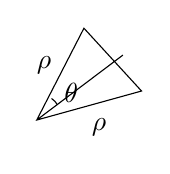
\begin{tikzpicture}[scale=.55]
\draw (0,0)--(1.09,2.12)--(2.42,.67)--cycle (0,0)--(1.99,1.50);
\draw (.48,.35) arc (30:56:.45);
\node at (.8,.63) {$\theta$}; \node[below] at (1.44,.25) {$\rho$}; \node[left] at (.56,1.26) {$\deleted{\unsure{\rho}}$};
\end{tikzpicture}}
\[
 2\rho\sin\tfrac{\theta}{2} \qquad G/H=X\ \underset{e}{\ni}
\]
\figure{\begin{tikzpicture}[scale=.70,line join=round]
\draw[thick] (0,0)--(2.2,3.0)--(2.34,1.0)--(4.93,1.35)--cycle;
\draw[very thick] (0,0)--(2.34,1.0) (2.34,1.0) .. controls (3.24,1.57) and (4.09,1.54) .. (4.93,1.35);
\draw (2.2,3.0) .. controls (2.66,2.33) and (2.51,1.72) .. (2.34,1.0);
\draw[->] (2.34,1.0)--(2.91,2.65); \draw[->] (2.34,1.0)--(3.99,2.01);
\draw[->] (2.22,2.04) .. controls (1.77,1.70) and (.74,2.19) .. (.48,2.88);
\node[left] at (.47,2.87) {$2\sin\tfrac{\alpha}{2}$}; \node at (3.28,2.24) {$72^\circ$};
\node at (1.15,.76) {$1\unsure{\alpha}$}; \node at (1.99,1.92) {$\unsure{\cos}$}; \node at (3.62,.94) {$\cos\alpha$};
\end{tikzpicture}}
\[
 \begin{aligned}
 \cos^2\alpha\cos\tfrac{2\pi}{5}&=\cos\alpha\\
 2\deleted{\unsure{\sin}}\sin\tfrac{\alpha}{2}\sin\tfrac{2\pi}{5}&=1
 \end{aligned}
\qquad
 \boxed{\cos\alpha=\frac{1}{2\sin^2\frac{2\pi}{\unsure{10|5}}}}
\]
\[
 \begin{aligned}
 \unsure{\gamma|y}e&=a.e=\dot a\\
 \gamma x&=\gamma ge=g'ue=g'\unsure{v|u|a}e=\deleted{\unsure{g'}} 
 \end{aligned}
\]
\figure{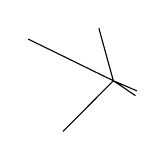
\begin{tikzpicture}[scale=.46]
\draw (0,0)--(2.35,-1.15)--(3,-1.43) (1.95,.30)--(2.35,-1.15)--(2.96,-1.56) (2.35,-1.15)--(.96,-2.55);
\end{tikzpicture}}
\[
 \begin{aligned}
 &\deleted{\unsure{bh}}\qquad b'=bh\\
 &b^{-1}b'\in H\\
 &\Rightarrow (ba)^{-1}b'a\in H\\
 &\text{i.e.}\quad a^{-1}b^{-1}b'a\subset H\\
 &\text{i.e.}\quad a^{-1}Ha\in H
 \end{aligned}
\]
% long diagonal strokes run through the calculation
\[
 1+x+x^2+x^3+x^4=0
\]
% margin note written sideways
\margin{$g(\sigma.i)$
$\begin{array}{ccccc}1&2&3&4&\deleted{5}\\ \hline 2&4&1&3&0\\ \hline 3&1&4&2&0\\ \hline\end{array}$\par
$p(g,\sigma.i)=(p(g),\sigma\unsure{)})(\unsure{\varphi|\rho}(1),\unsure{i})$
\par $\underset{\unsure{E}}{g}(\sigma{i})=g\sigma g^{-1}\quad g\unsure{\sigma'|r'|i}$}
% margin note written sideways
\margin{$\xi\quad\xi^2.\quad u,2u,3u,4u,0 \qquad \xi^i\quad G_{i,0}\quad e^{i\theta}$\par
$\left\{\begin{aligned}u^2+w^2&=1\\[-1pt]&\end{aligned}\right.\quad
\begin{pmatrix}\cos\theta&\unsure{u}\\ &\end{pmatrix}=$\par
$\unsure{\mathrm{II}}\quad\theta^2+\mu^2=1\qquad x^2-y^2$\par
$\begin{array}{ccc} G/\unsure{H} &\longrightarrow&G/H\\ \shortparallel&&\shortparallel\\ X&\longrightarrow&X\end{array}
\qquad \unsure{H}^{\unsure{\varphi}}\subset H$\par
$\begin{pmatrix}u&-v\\v&u\end{pmatrix}=\unsure{q}\begin{pmatrix}1&0\\0&1\end{pmatrix}$}
\figure{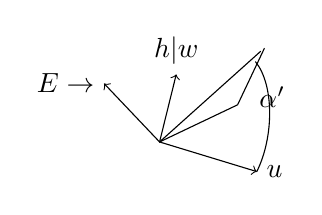
\begin{tikzpicture}[scale=.53,line join=round,line cap=round]
\coordinate (p) at (0,0); \draw[->] (p)--(-1.33,1.4) node[left] {$\unsure{E}\to$};
\draw[->] (p)--(.4,1.62) node[above] {$\unsure{h|w}$}; \draw (p)--(2.42,2.17);
\draw[->] (p)--(2.33,-.71) node[right] {$u$}; \draw (2.33,-.71) .. controls (2.75,.14) and (2.74,1.38) .. (2.30,1.92);
\draw (p)--(1.87,.89)--(2.51,2.24); \node at (2.70,1.07) {$\unsure{\alpha'}$};
\end{tikzpicture}}
\[
 \frac{N(H)}{\bigcap\text{conj.}\,H}\qquad
 \left(2\sin\tfrac{\alpha}{2}\right)\left(2\sin\unsure{>|{}^2} \tfrac{\pi}{4}\right)
\]
\figure{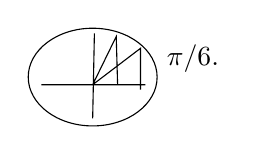
\begin{tikzpicture}[scale=.44]
\draw (0,0) ellipse (1.86 and 1.41);
\draw (0,-1.19)--(.05,1.26) (-1.48,-.22)--(1.52,-.22) (0,-.22)--(1.38,.83)--(1.38,-.36) (0,-.22)--(.68,1.17)--(.72,-.23);
\node[right] at (1.86,.53) {$\pi/6$.};
\end{tikzpicture}}
\[
 \begin{aligned}
 \alpha&=60\,?\\
 \cos\tfrac{\alpha}{2}&=\tfrac{\sqrt3}{2}\\
 \sqrt3\sin\tfrac{\pi}{5}&=1
 \end{aligned}
\]
\figure{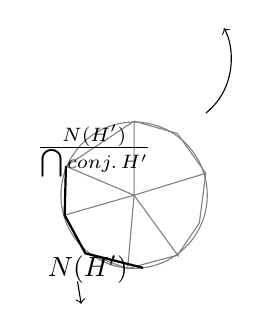
\begin{tikzpicture}[scale=.57, line join=round]
\draw[gray] (0,0) circle (1.63);
\draw[gray] (90:1.65)--(55:1.68)--(17:1.67)--(-23:1.58)--(-54:1.65)--(-95:1.64)--(-130:1.69)--(-164:1.61)--(157:1.65)--cycle;
\draw[gray] (0,0)--(90:1.65) (0,0)--(17:1.66) (0,0)--(-54:1.69) (0,0)--(-95:1.64) (0,0)--(-164:1.61) (0,0)--(157:1.65);
\draw[thick] (157:1.65)--(-164:1.61)--(-130:1.69)--(-83:1.63);
\node at (-.89,.98) {$\frac{N(H')}{\bigcap\text{conj.}\,H'}$}; \node at (-1.03,-1.65) {$N(\unsure{H'})$};
\draw[->] (1.6,1.83) .. controls (2.31,2.4) and (2.23,3.35) .. (2.0,3.72);
\draw[->] (-1.26,-1.92)--(-1.18,-2.42);
\end{tikzpicture}}
\[
 \begin{array}{ccccccc}
 N(H)\cap N(H')&=&N(H\cap H')&\subset&N(H)&=&\mathbb Z_3.\mathbb F_2^2\\
 &&\cup&&\cup\\
 &&H'&\subset&H&\text{---}&\mathbb F_2^2\\
 &&\cup&&\cup\\
 K\cap H'&=&\underset{0}{K'}&\subset&K&=&0
 \end{array}
\]
% archive sheet number: 19
